\documentclass[12pt,a4paper]{article}

\usepackage[utf8]{inputenc}
\usepackage[T1]{fontenc}
\usepackage[spanish,es-nodecimaldot]{babel}
\usepackage{lmodern}
\usepackage{geometry}
\usepackage{graphicx}
\usepackage{array}
\usepackage{amsmath}
\usepackage{booktabs}
\usepackage{longtable}
\usepackage{xcolor}
\usepackage{hyperref}
\usepackage{fancyhdr}
\usepackage{tikz}
\usepackage{pgfplots}
\pgfplotsset{compat=1.18}

\geometry{top=2.5cm,bottom=2.5cm,left=2.7cm,right=2.7cm}
\hypersetup{colorlinks=true,linkcolor=black,urlcolor=blue}
\definecolor{azulGestion}{RGB}{31,78,121}
\definecolor{grisSuave}{RGB}{245,247,250}

\pagestyle{fancy}
\fancyhf{}
\fancyhead[L]{\small GestionCapa}
\fancyhead[R]{\small Laboratorio 08}
\fancyfoot[C]{\thepage}
\setlength{\headheight}{15pt}

\begin{document}

\begin{titlepage}
\centering
\vspace*{0.8cm}
{\Large\textbf{UNIVERSIDAD NACIONAL DE SAN ANTONIO ABAD DEL CUSCO}\par}
\vspace{0.3cm}
{\large FACULTAD DE INGENIERÍA ELÉCTRICA, ELECTRÓNICA, INFORMÁTICA Y MECÁNICA\par}
\vspace{0.3cm}
{\large ESCUELA PROFESIONAL DE INGENIERÍA INFORMÁTICA Y DE SISTEMAS\par}
\vspace{0.4cm}

\includegraphics[width=3.2cm]{capturasJira/escudoUnsaac.png}\par
\vspace{0.8cm}
\vfill
{\Large\textbf{INFORME DE LABORATORIO}\par}
\vspace{0.5cm}
{\Huge\textbf{LABORATORIO 08}\par}
\vspace{0.3cm}
{\LARGE\textbf{Burndown Chart}\par}
\vspace{0.8cm}
{\large\textbf{Proyecto:} GestionCapa -- Gestión de capacitaciones del Colegio Profesional de Profesores del Perú -- Región Cusco\par}
\vfill
\begin{flushleft}
\textbf{Curso:} Ingeniería de Software I\\
\textbf{Docente:} Lisha Sabah Diaz Caceres\\[0.3cm]
\textbf{Integrantes:}\\
Wilfredo Chino Choquenaira (141002)\\
Luz Diana Ancasi Aymachoque (215714)\\
Mirian Lucero Ancco Ancalla (225416)\\
Efrain Vitorino Marin (160337)\\
Hernan Washington Ramos Alata (221989)\\[0.3cm]
\textbf{Semestre:} 2026-2
\end{flushleft}
\vfill
{\large CUSCO -- PERÚ\par}
{\large 2026\par}
\end{titlepage}

\tableofcontents
\newpage

\section{Objetivo}

Monitorear el avance del Sprint 3 de GestionCapa mediante el uso de métricas
ágiles, construyendo e interpretando un Burndown Chart que compare el trabajo
ideal con el trabajo real pendiente y permita detectar desviaciones durante el
sprint.

\section{Fundamento teórico}

\subsection{Métricas ágiles}

Las métricas ágiles son indicadores que ayudan al equipo Scrum a conocer el
estado del trabajo, evaluar su capacidad y tomar decisiones oportunas. Deben
interpretarse junto con la comunicación del equipo, la calidad del producto y
el cumplimiento de la Definition of Done.

\subsection{Burndown Chart}

El Burndown Chart muestra los story points pendientes en función del tiempo.
El eje horizontal representa los días del sprint y el eje vertical representa
los puntos restantes. La línea ideal disminuye uniformemente desde el total
comprometido hasta cero; la línea real disminuye cuando las historias cumplen
la Definition of Done.

\subsection{Velocidad del equipo}

La velocidad es la cantidad de story points que el equipo termina en un
sprint. Sirve para planificar la capacidad de sprints posteriores, pero no
debe utilizarse para comparar equipos distintos. En GestionCapa, la velocidad
de referencia documentada para el Sprint 1 fue de 58 puntos.

\subsection{Seguimiento del progreso}

El seguimiento se realiza revisando diariamente el tablero, los estados de
las historias y el Burndown. Si la línea real está por encima de la ideal,
existe retraso; si está por debajo, existe adelanto. Un tramo horizontal
indica que no se terminaron historias con puntos durante ese período. Una
subida puede indicar incorporación de alcance o reapertura de trabajo.

\section{Herramientas}

\begin{itemize}
    \item \textbf{Jira Software:} registro del Sprint 3, historias, épicas,
    story points, estados y fechas de finalización.
    \item \textbf{Excel:} tabla de puntos restantes y gráfico del archivo
    \texttt{Burndown\_Sprint3\_GestionCapa.xlsx}.
    \item \textbf{GitHub:} control de versiones del proyecto GestionCapa.
\end{itemize}

\section{Actividades}

\subsection{Parte 1: Introducción al Burndown}

\subsubsection{Qué mide}

Mide los story points que faltan terminar en cada día del sprint. Solo se
descuentan los puntos de historias que pasan a ``Hecho''. Una historia
parcialmente avanzada conserva sus puntos pendientes hasta cumplir todos sus
criterios de aceptación.

\subsubsection{Cómo se interpreta}

\begin{itemize}
    \item Línea real por encima de la ideal: el equipo está retrasado.
    \item Línea real por debajo de la ideal: el equipo está adelantado.
    \item Líneas coincidentes: el avance sigue el ritmo previsto.
    \item Línea horizontal: no se cerraron historias con puntos.
    \item Subida de la línea real: se agregó trabajo o se reabrió una historia.
\end{itemize}

\subsection{Parte 2: Construcción del gráfico}

\subsubsection{Datos del Sprint 3}

El Sprint 3 se desarrolla del 09/11/2026 al 20/11/2026, con una duración de
12 días calendario. El objetivo es que un docente conozca el curso mediante
un enlace compartido, se inscriba como colegiado o externo, pague según la
modalidad y asista de forma presencial, virtual o híbrida, con asistencia
registrada y constancia emitida según las reglas del curso.

\begin{table}[h]
\centering
\caption{Datos generales del Sprint 3}
\label{tab:datosSprint3}
\begin{tabular}{p{5cm}p{8.5cm}}
\toprule
\textbf{Elemento} & \textbf{Dato}\\
\midrule
Sprint & Sprint 3\\
Fechas & 09/11/2026 -- 20/11/2026\\
Actividades registradas & 15\\
Puntos comprometidos & 11 story points\\
Fecha de corte & 16/11/2026, día 8\\
Estado al corte & 8 de 11 puntos completados; 3 puntos pendientes\\
\bottomrule
\end{tabular}
\end{table}

\subsubsection{Historias estimadas}

\begin{table}[h]
\centering
\caption{Historias con story points del Sprint 3}
\label{tab:historiasSprint3}
\begin{tabular}{p{2cm}p{6.5cm}p{2.3cm}p{3cm}}
\toprule
\textbf{Código} & \textbf{Historia} & \textbf{Puntos} & \textbf{Estado al corte}\\
\midrule
HU-22 & Página pública de cursos del subdominio & 2 & Hecho\\
HU-26 & Sesiones virtuales seguras & 3 & Hecho\\
HU-29 & Notificaciones por correo & 3 & Pendiente\\
HU-32 & Pago por transferencia BCP y en efectivo & 3 & Hecho\\
\midrule
\multicolumn{2}{r}{\textbf{Total}} & \textbf{11} & \\
\bottomrule
\end{tabular}
\end{table}

Además de estas historias estimadas, el sprint contiene elementos sin
estimación. Por ello, el Burndown refleja únicamente los 11 story points y no
todo el volumen de actividades del sprint. El HTML de seguimiento identifica
los siguientes 11 elementos sin estimar: HU-36, HU-39, HU-40, HU-43, HU-51,
HU-53, HU-54, T-20, T-21, T-24 y T-25.

\subsubsection{Cálculo de la línea ideal}

Para un sprint de 12 días y 11 puntos comprometidos, la reducción ideal diaria
es de un punto. La fórmula utilizada es:

\[
\text{Puntos ideales del día }d =
11 - 11\left(\frac{d-1}{11}\right)
\]

\begin{table}[h]
\centering
\caption{Puntos restantes del Sprint 3}
\label{tab:burndownSprint3}
\begin{tabular}{>{\centering\arraybackslash}p{1.5cm}
                >{\centering\arraybackslash}p{2.5cm}
                >{\centering\arraybackslash}p{2.5cm}
                >{\centering\arraybackslash}p{2.8cm}
                >{\centering\arraybackslash}p{3cm}}
\toprule
\textbf{Día} & \textbf{Fecha} & \textbf{Ideal} & \textbf{Real} & \textbf{Real -- ideal}\\
\midrule
1 & 09/11 & 11 & 11 & 0\\
2 & 10/11 & 10 & 11 & +1\\
3 & 11/11 & 9 & 11 & +2\\
4 & 12/11 & 8 & 11 & +3\\
5 & 13/11 & 7 & 11 & +4\\
6 & 14/11 & 6 & 9 & +3\\
7 & 15/11 & 5 & 6 & +1\\
8 & 16/11 & 4 & 3 & -1\\
9 & 17/11 & 3 & -- & --\\
10 & 18/11 & 2 & -- & --\\
11 & 19/11 & 1 & -- & --\\
12 & 20/11 & 0 & -- & --\\
\bottomrule
\end{tabular}
\end{table}

\begin{figure}[h]
\centering
\begin{tikzpicture}
\begin{axis}[
    width=0.93\textwidth,
    height=8cm,
    xlabel={Día del sprint},
    ylabel={Story points restantes},
    xmin=1, xmax=12,
    ymin=0, ymax=12,
    xtick={1,2,3,4,5,6,7,8,9,10,11,12},
    ytick={0,1,2,3,4,5,6,7,8,9,10,11},
    grid=both,
    legend style={at={(0.5,-0.2)},anchor=north,legend columns=2},
    line width=1.2pt
]
\addplot[color=orange, dashed, mark=none]
    coordinates {(1,11) (2,10) (3,9) (4,8) (5,7) (6,6)
                 (7,5) (8,4) (9,3) (10,2) (11,1) (12,0)};
\addlegendentry{Línea ideal}
\addplot[color=blue, mark=*, mark size=2pt]
    coordinates {(1,11) (2,11) (3,11) (4,11) (5,11)
                 (6,9) (7,6) (8,3)};
\addlegendentry{Avance real}
\addplot[color=red, dashed, mark=none]
    coordinates {(8,0) (8,12)};
\addlegendentry{Corte: 16/11}
\end{axis}
\end{tikzpicture}
\caption{Burndown Chart del Sprint 3 al 16/11/2026}
\label{fig:burndownSprint3}
\end{figure}

\begin{figure}[h]
\centering
\begin{tikzpicture}
\begin{axis}[
    ybar,
    width=0.93\textwidth,
    height=7cm,
    bar width=13pt,
    xlabel={Día del sprint},
    ylabel={Story points terminados acumulados},
    xmin=0.4, xmax=8.6,
    ymin=0, ymax=9,
    xtick={1,2,3,4,5,6,7,8},
    ytick={0,2,4,6,8},
    grid=major,
    nodes near coords,
    every node near coord/.append style={font=\small}
]
\addplot[fill=azulGestion!70] coordinates
    {(1,0) (2,0) (3,0) (4,0) (5,0) (6,2) (7,5) (8,8)};
\end{axis}
\end{tikzpicture}
\caption{Puntos terminados acumulados según la tabla del Excel}
\label{fig:avanceAcumulado}
\end{figure}

\subsection{Parte 3: Análisis}

\begin{table}[h]
\centering
\caption{Comparación entre línea ideal y avance real}
\label{tab:analisisSprint3}
\begin{tabular}{p{3.4cm}p{5cm}p{5cm}}
\toprule
\textbf{Tramo} & \textbf{Comportamiento observado} & \textbf{Interpretación}\\
\midrule
Días 1--5 & La línea real permanece en 11 puntos mientras la ideal disminuye
hasta 7. & Retraso creciente de hasta 4 puntos; no se cerraron historias
estimadas durante la primera semana.\\
Días 6--8 & La línea real disminuye de 11 a 3 puntos y cruza la ideal en el
día 8. & Se recupera el retraso y el sprint queda 1 punto adelantado al corte.\\
15/11 & HU-22 se reabre y vuelve a cerrarse el mismo día. & Existe trabajo
rehecho; el primer cierre no cumplía completamente la Definition of Done.\\
Alcance total & Solo 4 de 15 actividades tienen story points. & El Burndown
muestra 8 de 11 puntos completados, pero no refleja los elementos sin estimar.\\
\bottomrule
\end{tabular}
\end{table}

Al corte del 16/11/2026 se han completado 8 de 11 story points, equivalente al
72.7\% del trabajo estimado. La línea real está un punto por debajo de la
ideal, pero esta conclusión debe limitarse a los elementos estimados. En
términos de elementos, se han completado 7 de 15 actividades, equivalente al
46.7\%. La diferencia se explica porque 11 actividades no tienen story points y
no aparecen en el Burndown; por tanto, el gráfico puede sobreestimar el avance
real del sprint.

Para los días 9 a 12, la proyección conserva tres puntos pendientes
correspondientes a HU-29, mientras que los elementos sin estimar deben
continuar controlándose directamente en Jira. En particular, el HTML registra
HU-36 en desarrollo y otros elementos todavía pendientes, lo que confirma que
el Burndown debe complementarse con el tablero y no utilizarse como único
indicador.

\section{Entregable}

\begin{table}[h]
\centering
\caption{Entregables y evidencias}
\label{tab:entregables}
\begin{tabular}{p{5cm}p{8.5cm}}
\toprule
\textbf{Entregable} & \textbf{Evidencia}\\
\midrule
Burndown Chart & Tabla~\ref{tab:burndownSprint3}, Figura~\ref{fig:burndownSprint3}
y archivo \texttt{Burndown\_Sprint3\_GestionCapa.xlsx}.\\
Análisis del avance & Tabla~\ref{tab:analisisSprint3} y explicación del
comportamiento al corte.\\
Evidencia de Jira & Capturas del backlog, épicas, estados y resumen del
proyecto incluidas en las Figuras~\ref{fig:backlogJira} y
\ref{fig:resumenJira}.\\
\bottomrule
\end{tabular}
\end{table}

\begin{figure}[h]
\centering
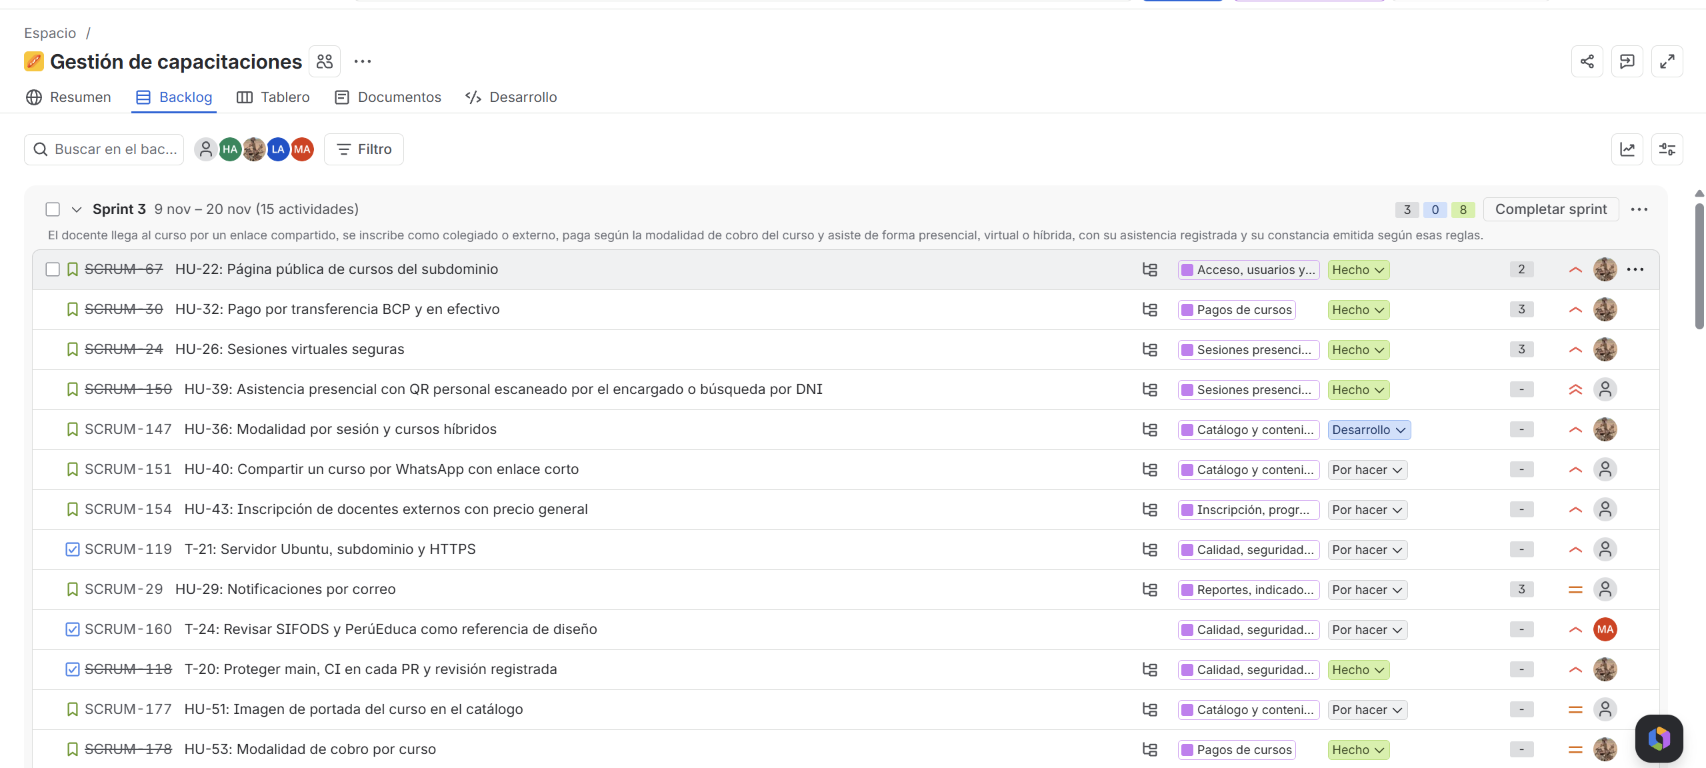
\includegraphics[width=\textwidth]{capturasJira/capturaBacklogSprint3.png}
\caption{Backlog de Jira con actividades, épicas, estados y story points}
\label{fig:backlogJira}
\end{figure}

\begin{figure}[h]
\centering
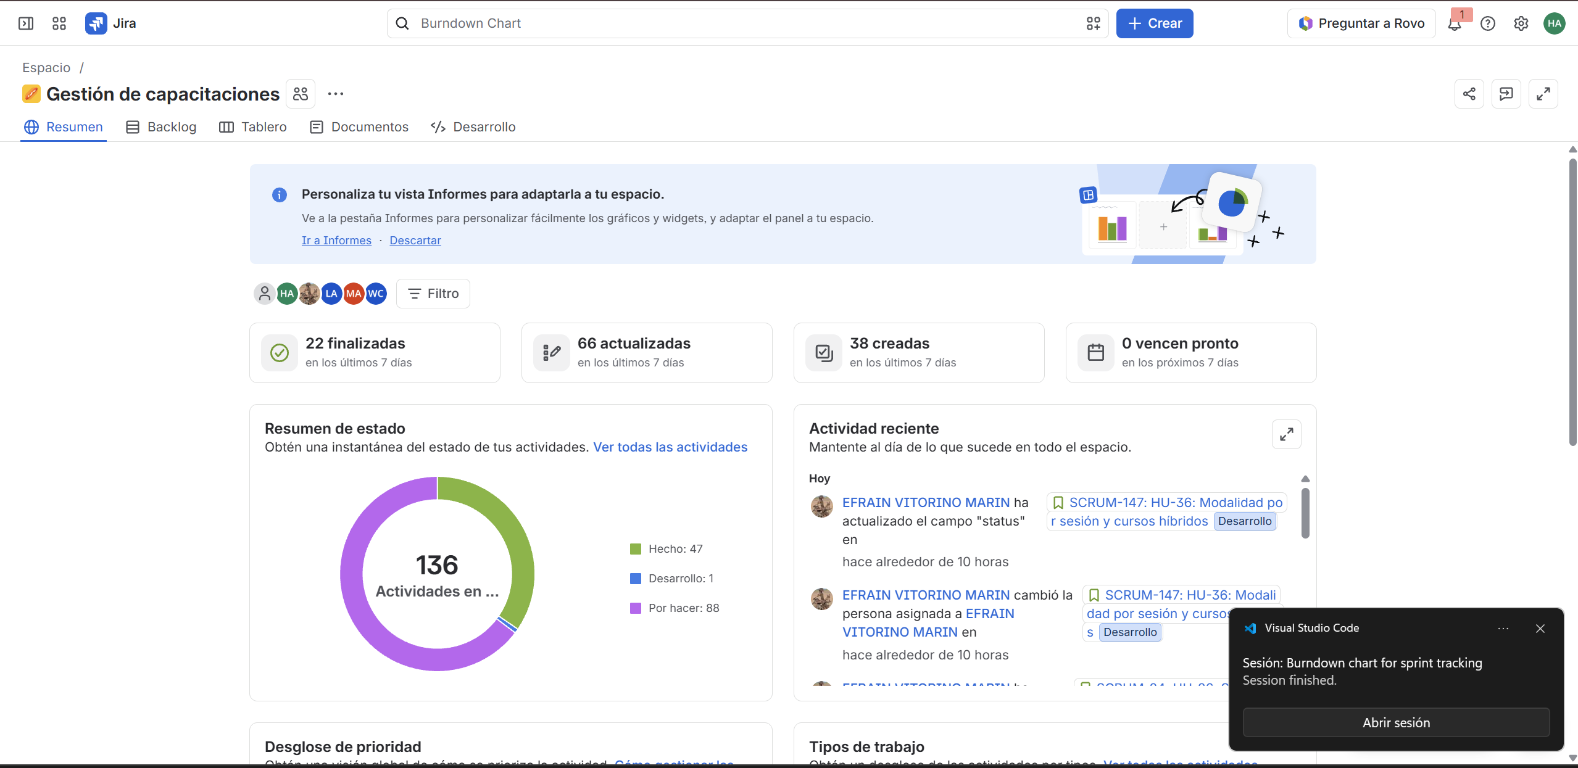
\includegraphics[width=\textwidth]{capturasJira/capturaResumenJira.png}
\caption{Resumen del proyecto GestionCapa en Jira}
\label{fig:resumenJira}
\end{figure}

\begin{figure}[h]
\centering
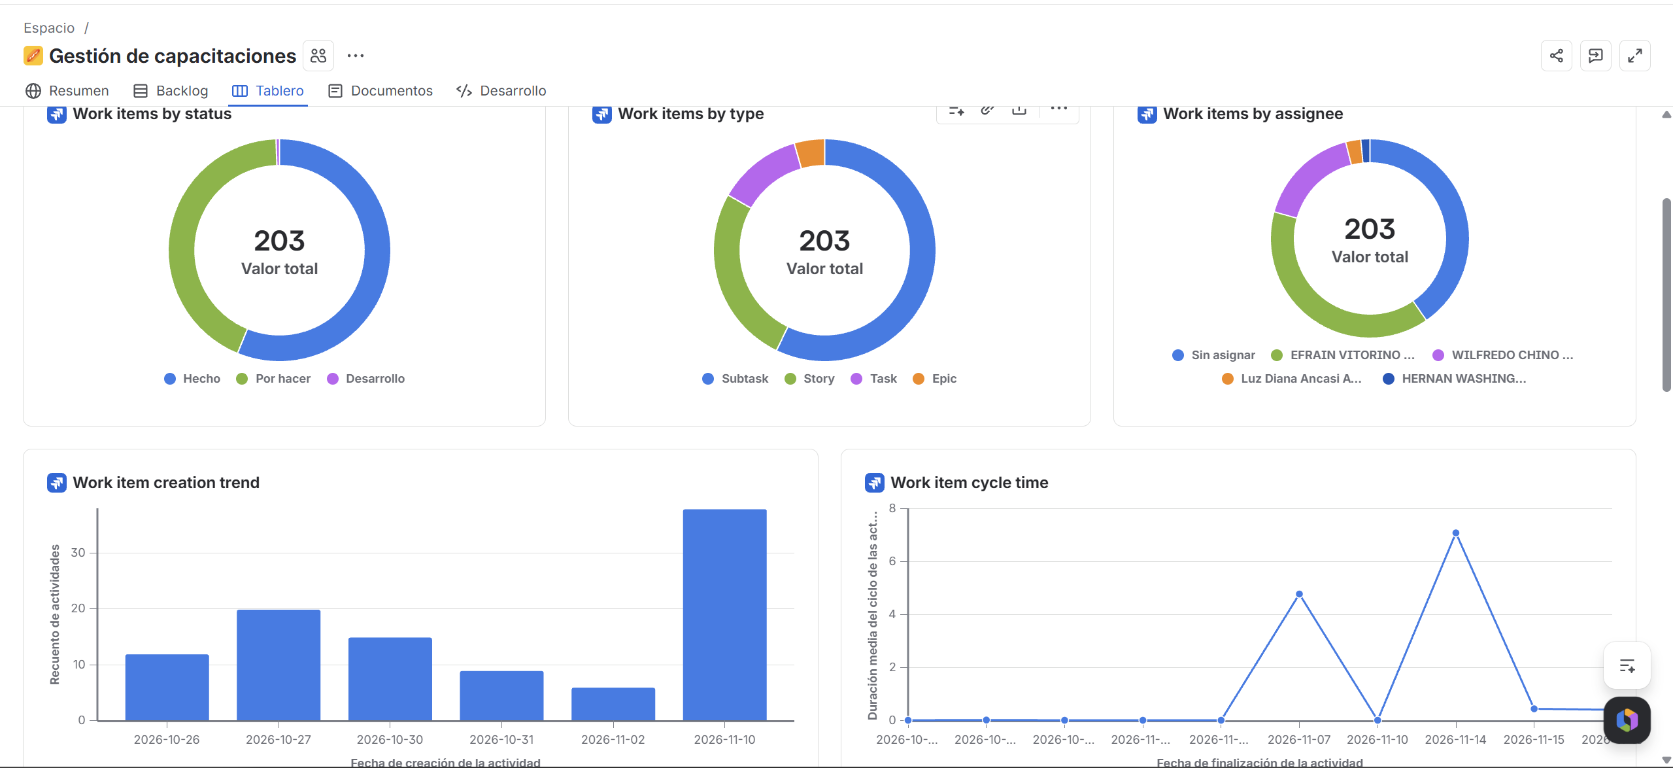
\includegraphics[width=\textwidth]{capturasJira/capturaPanelMetricasJira.png}
\caption{Panel de Jira: distribución de elementos por estado, tipo y responsable}
\label{fig:panelMetricasJira}
\end{figure}

\begin{figure}[h]
\centering
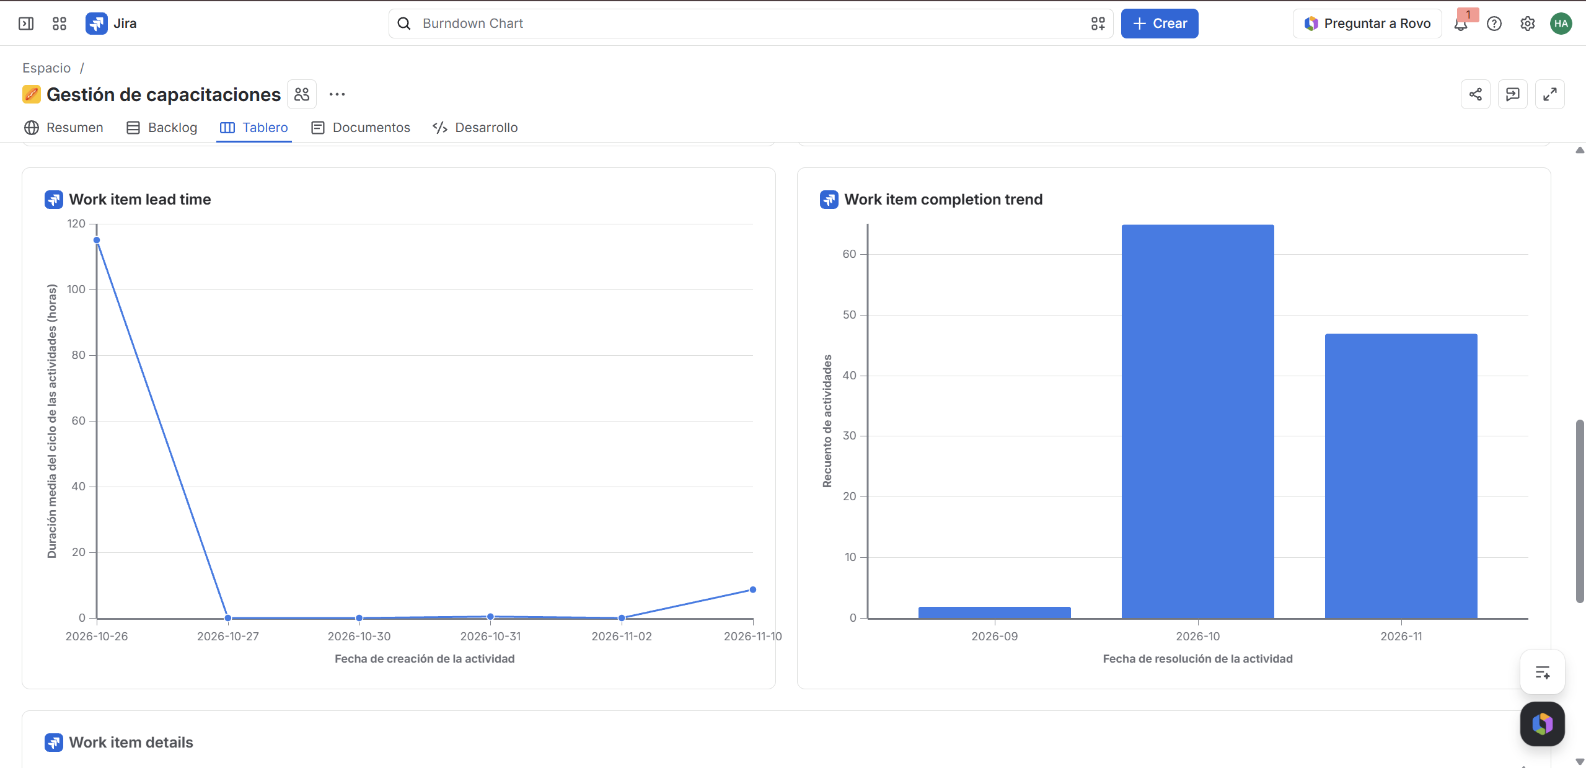
\includegraphics[width=\textwidth]{capturasJira/capturaMetricasTendenciasJira.png}
\caption{Panel de Jira: tiempo de ciclo, tiempo de entrega y tendencia de finalización}
\label{fig:tendenciasJira}
\end{figure}

\begin{figure}[h]
\centering
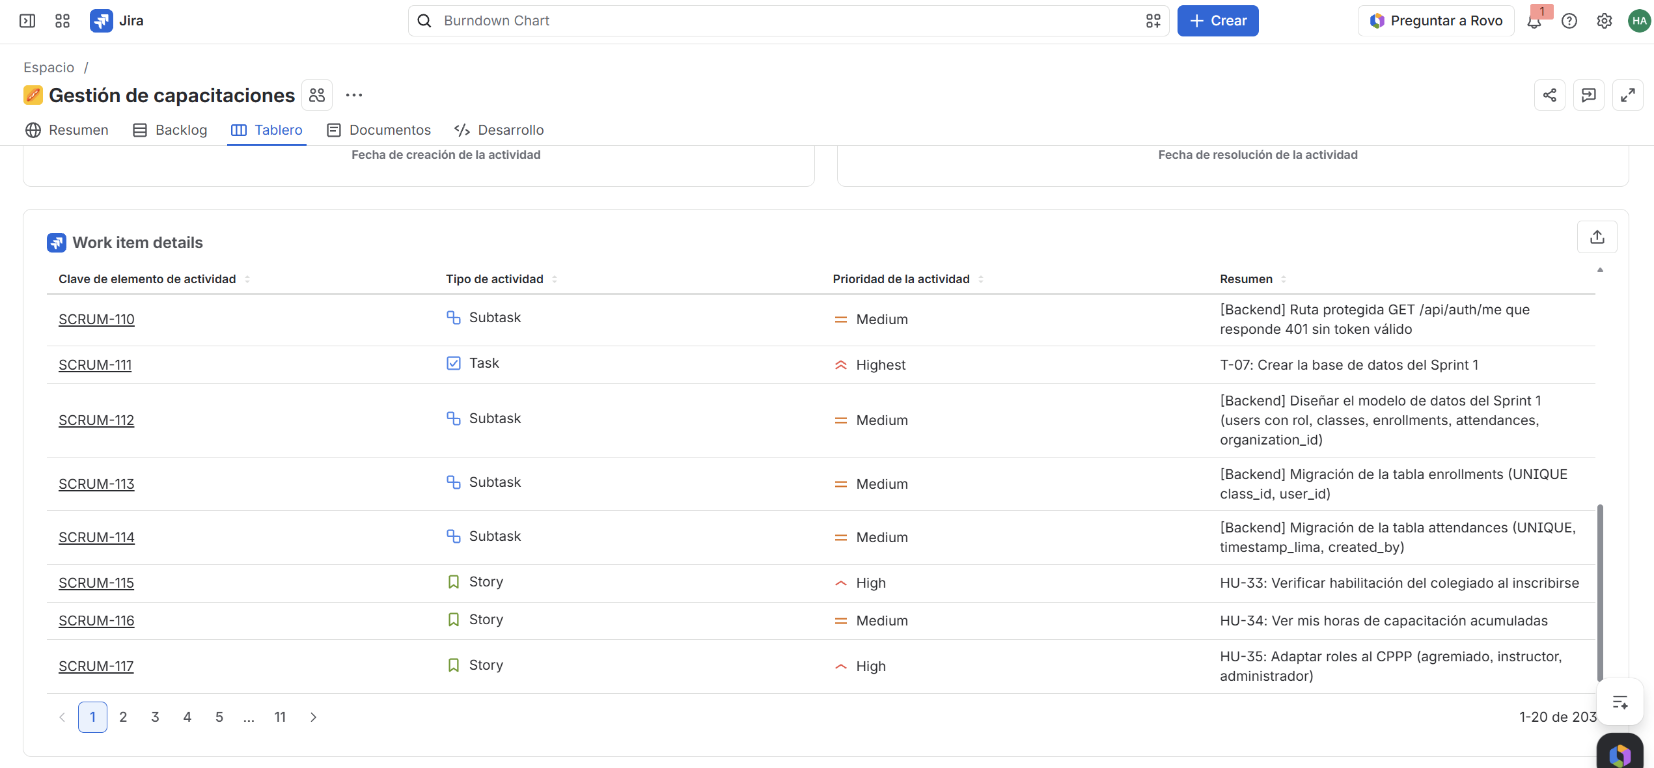
\includegraphics[width=\textwidth]{capturasJira/capturaDetalleTrabajoJira.png}
\caption{Detalle de elementos de trabajo registrados en Jira}
\label{fig:detalleJira}
\end{figure}

\noindent
Las capturas complementan el Burndown: el panel de métricas permite observar
la distribución general del trabajo, las tendencias muestran el comportamiento
temporal de las actividades y el detalle permite verificar que Jira contiene
historias, tareas y subtareas con sus prioridades y descripciones.

\section{Trabajo extra: actualización diaria del gráfico}

\begin{table}[h]
\centering
\caption{Registro diario del Sprint 3 al 16/11/2026}
\label{tab:registroDiario}
\begin{tabular}{p{2cm}p{8cm}p{3cm}}
\toprule
\textbf{Fecha} & \textbf{Cambios registrados en Jira} & \textbf{Puntos restantes}\\
\midrule
09/11 & Inicio del sprint. & 11\\
10/11 & Se cargan las historias del sprint; no se termina una historia con
puntos. & 11\\
11/11 & Sin historias estimadas terminadas. & 11\\
12/11 & Sin historias estimadas terminadas. & 11\\
13/11 & Sin historias estimadas terminadas. & 11\\
14/11 & Se termina HU-22 y una tarea sin puntos. & 9\\
15/11 & Se termina HU-32 y elementos sin puntos; HU-22 se reabre y se cierra
nuevamente. & 6\\
16/11 & Se termina HU-26; HU-36 pasa a desarrollo. & 3\\
\bottomrule
\end{tabular}
\end{table}

La actualización diaria debe continuar hasta el cierre del sprint. En cada
Daily Scrum se deben revisar los puntos restantes, los bloqueos y las
historias reabiertas. Si se agregan actividades, debe registrarse el cambio de
alcance y decidir si también serán estimadas para evitar que el Burndown
muestre una imagen incompleta del trabajo.

\section{Conclusiones}

\begin{itemize}
    \item El Burndown permitió identificar un retraso acumulado de cuatro
    puntos durante los primeros cinco días del Sprint 3.
    \item El equipo recuperó el retraso entre los días 6 y 8, llegando a tres
    puntos restantes frente a cuatro puntos ideales.
    \item Al corte se completó el 72.7\% de los story points estimados, pero
    solo cuatro de las quince actividades tenían estimación.
    \item La diferencia entre actividades y story points demuestra que el
    gráfico debe complementarse con el tablero y la revisión de alcance.
    \item La reapertura de HU-22 evidencia la importancia de validar la
    Definition of Done antes de cerrar una historia.
\end{itemize}

\section{Enlaces y fuentes del proyecto}

\begin{itemize}
    \item Repositorio: \url{https://github.com/lovito99/gestioncapa}
    \item Documentación del proyecto: \url{https://github.com/lovito99/gestioncapa/tree/main/docs}
    \item Archivo de datos: \texttt{Burndown\_Sprint3\_GestionCapa.xlsx}
\end{itemize}

\end{document}
